% !TeX root = ../SPL-Rules.tex
% !TeX spellcheck = en_US
\section{Technical Challenges}

\subsection{7 vs. 7}
    This competition extends the ideas from the mixed team competition, and 1 vs. 1 remote challenge from RoboCup 2021 to a standardized 7 vs. 7 on-site competition. Another goal is to enforce more collaborative game play. This challenge will only be executed if at least four teams participate.

    \subsubsection{Condition for participation}
    \label{sec:7vs7:condition_for_participation}
        \begin{itemize}
            \item A 7 vs. 7 team can be build from a single team but also from multiple teams.
            \item Teams need at least four own robots to play with.
            \item Teams have to provide three tested robots (\textbf{only V6 version}) to a robot pool.
            \item The pool robots have to be calibrated in limited time.
        \end{itemize}

    \subsubsection{Rules}
        This challenge bases on all rules from the 5 vs. 5 competition (\crefrange{sec:setup_environment}{sec:judgment}). The following list contains extended and changed rules for this challenge in order to ensure, among other things, the safety of pool robots:

        \paragraph{Players}
            In total each team consists of 7 players without a substitution robot. The 7 robots consist of 4 own and 3 pool robots. Whereby the pool robots are only V6s. Each jersey shirt has therefore now player numbers between 1 and 7 printed on it (\cf \cref{sec:team_markers}). Also the new positions of the initial kick-off (\cf \cref{sec:initial-kick-off}) for 7 robots can be seen in \cref{fig:initial_positions_7vs7}.
            \begin{figure}[t!]
            	\begin{center}
            		\leavevmode
            		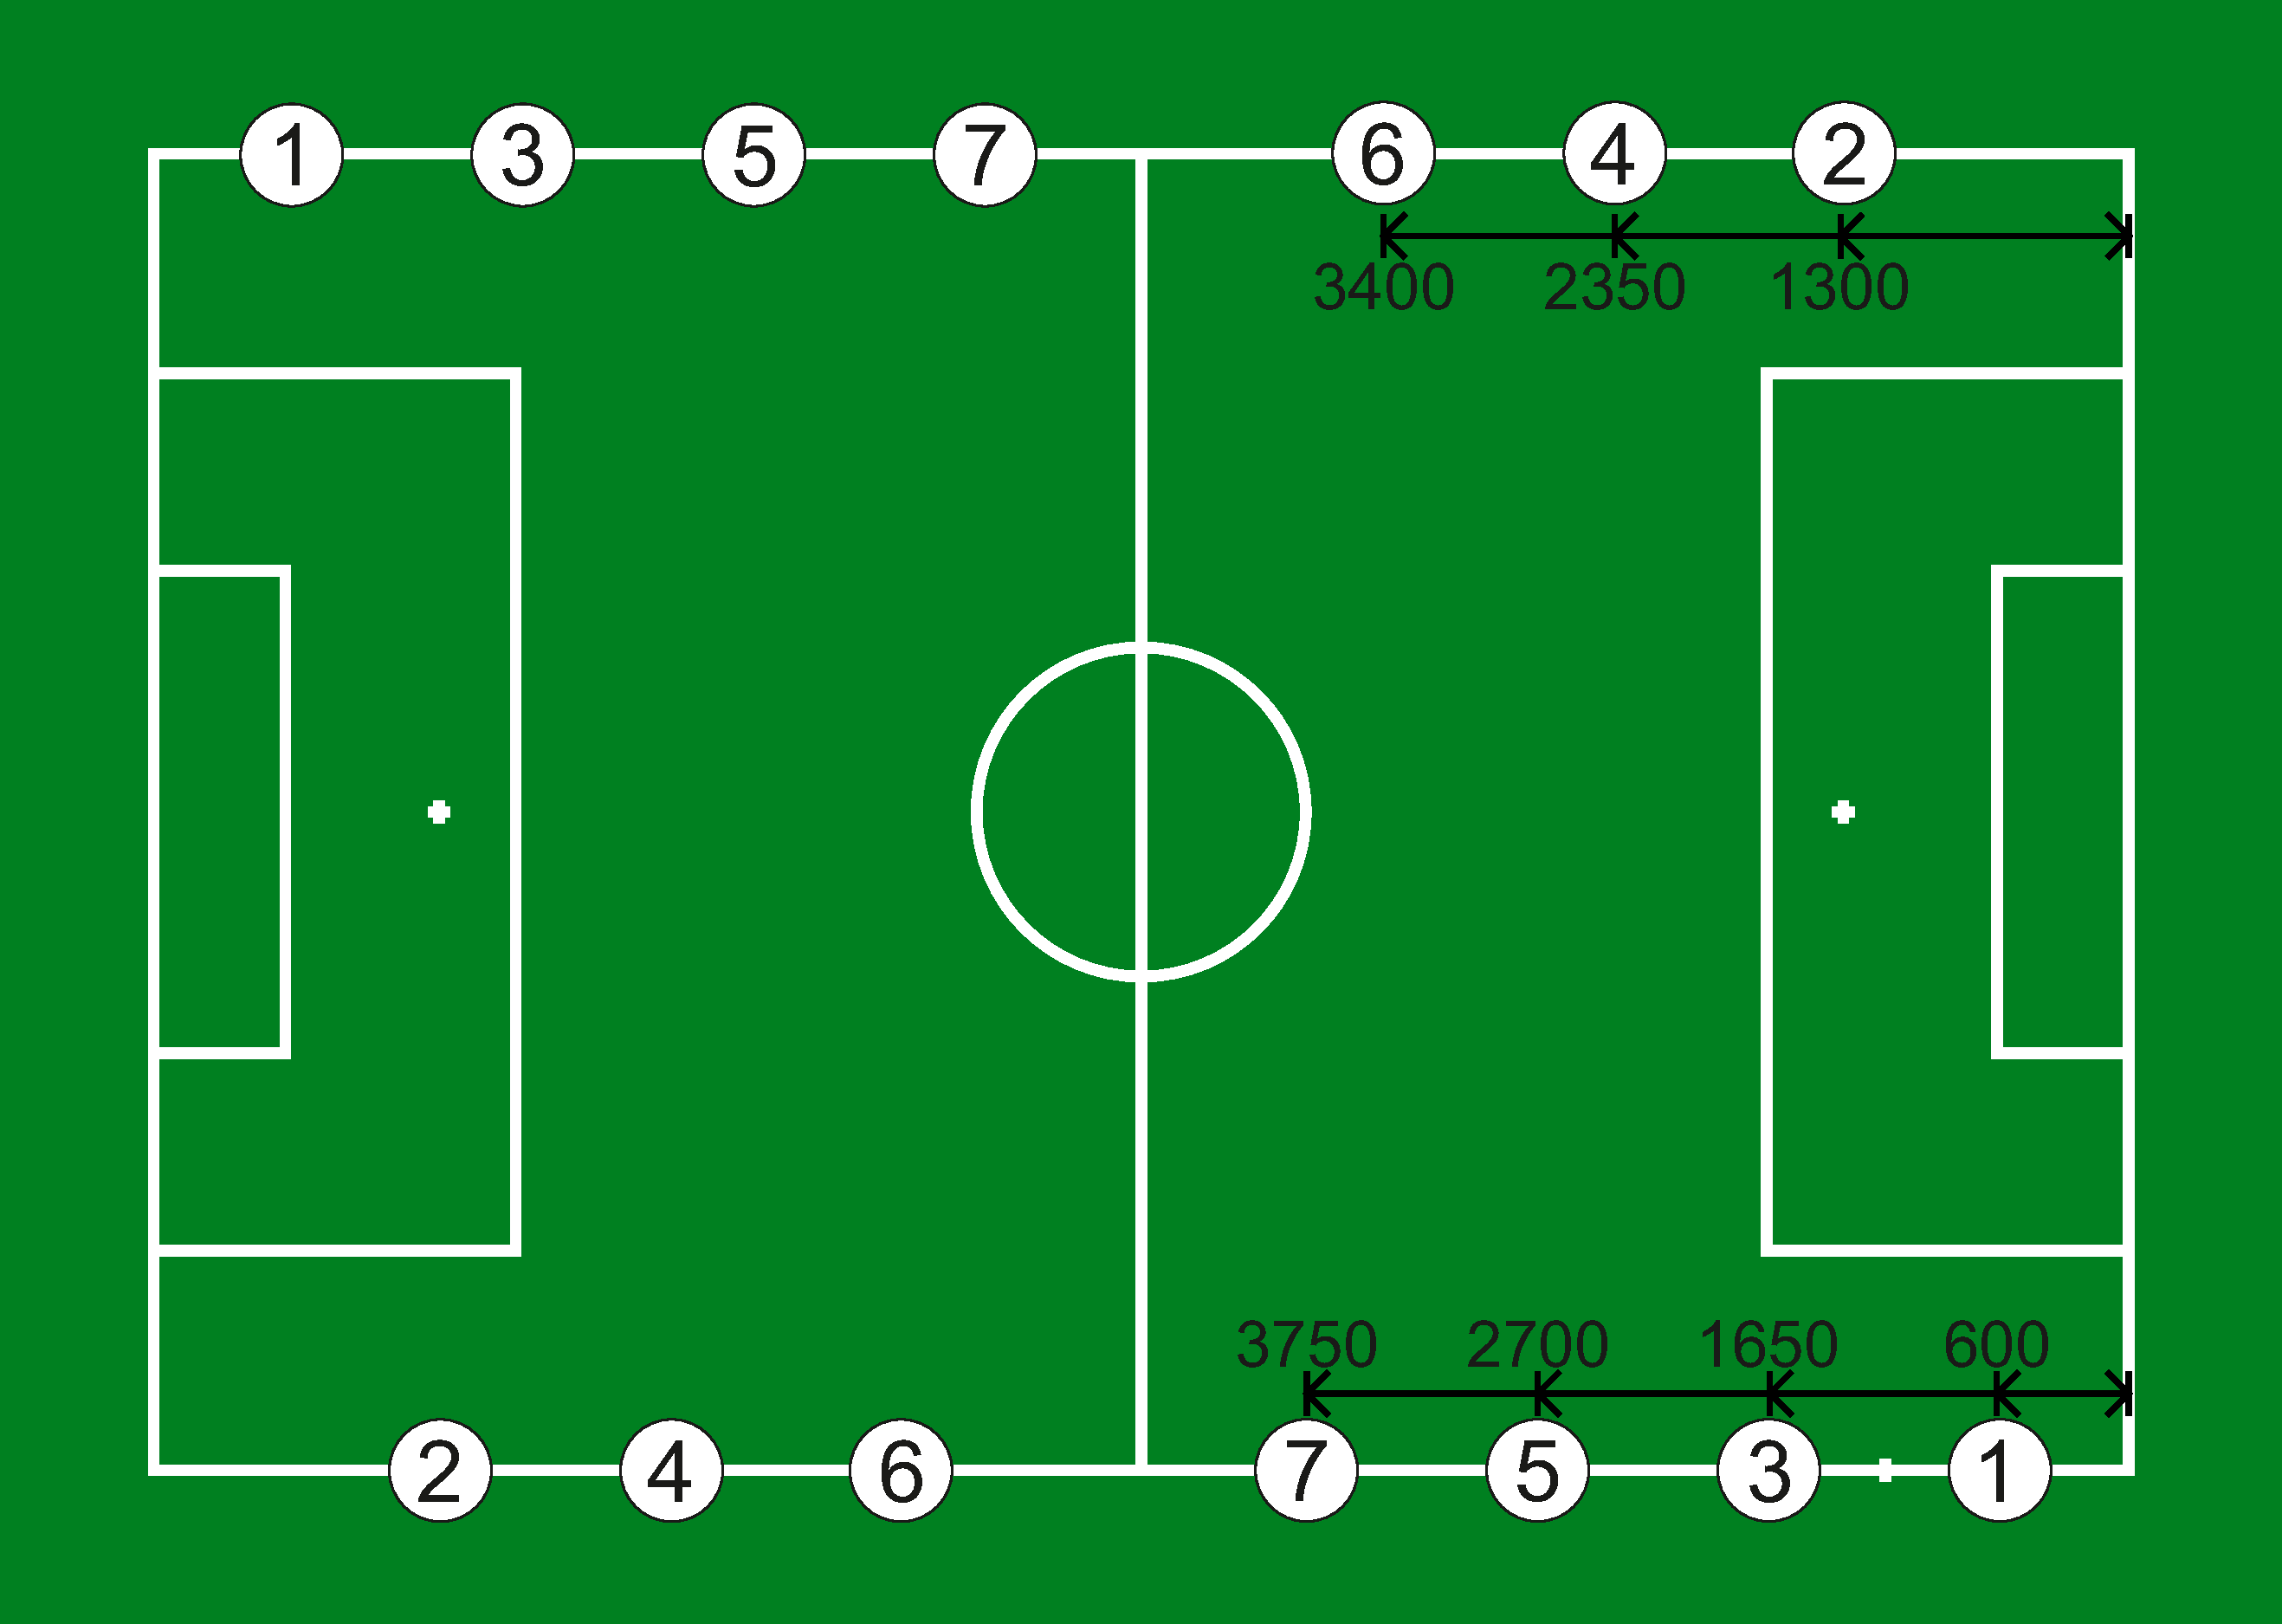
\includegraphics[width=1\columnwidth]{figs/initial_positions_7vs7.pdf}
            		\caption{Positions, player numbers and distances from the center of the goal line for the initial kick-off of the 7 vs. 7 robots.}
            		\label{fig:initial_positions_7vs7}
            	\end{center}
            \end{figure}

        \paragraph{Referees}
            \label{sec:7vs7:referee}
            All referees are allowed to prevent robots from crashing to the ground by catching them beforehand and then laying them down gently. Additionally the head referee decides whether a robot excessively damages itself and should remove it from the field via a forced “Request for Pick-up”, \cf \cref{sec:request_for_pickup}.

        \paragraph{Robot Pool}
            Each team has to contribute at least 3 robots to the robot pool, \cf \cref{sec:7vs7:condition_for_participation}. If a team cannot provide enough own robots and there are still functional robots in the robot pool, then this team can get more than the 3 robots from the pool to restock up to 7 robots. However, the final decision is still up to the head referee. \\
            The robot pool exists only virtually, so that there is no central location where all pool robots are stored. Each team is also allowed to use their own pool robots when they are not in use. However, each pool robot gets a unique ID and in order to be able to recognize the pool robots visually, a sticker is attached to the outer sides of the upper arms and on the back of the head.

        \paragraph{Robot Pool Evaluation}
            \label{sec:robot_pool_evaluation}
            In order to guarantee that the pool robots are functional, and all parts are working within their limits each team has to provide a proof of functionality one hour before a specific pool robot is planned for a game. Also, the team has to ensure that this robot had at least a cooldown period of \qty{15}{\minute} and is charged to at least \qty{80}{\percent}.
            A common robot evaluation image will be provided by the community with a standardized setup procedure (custom image) and with automatic calibration. Afterwards the robot should walk towards a ball and shoot it. If this evaluation is completed without any problems within a given time \todo{set time} and the robot falls down less than 2 times, the evaluation is to be rated as functional. Otherwise, this robot is considered to be non-functional for the time being. Every team can propose such an image up to the 2022-06-01\todo{set deadline}, as well as additional tests which should be included in such an evaluation image. A manual how to use the custom image should also be included.

        \paragraph{Hardware Related Penalties}
            \label{sec:7vs7:hardware_related_penalties}
            Since teams are partially playing with robots from other teams, there is a maximum of two hardware related penalties for each robot in the first half and one more in the second half.
            Hardware related penalties are:
            \begin{itemize}
                \item fallen robot or inactive robot, \cf \cref{sec:fallenrobots}
                \item request for pick-up in the playing or ready state — either by the team or forced by the head referee, \cf \cref{sec:request_for_pickup} and \cref{sec:7vs7:referee}.
            \end{itemize}
            These penalties are counted by the GameController operator and after that a robot with additional hardware related penalties is excluded for the rest of the game (they are transitioned into the unstiffed state by the assistant referees, \cf \cref{sec:robot_states})!

        \paragraph{Own Pushing}
            In addition to the normal pushing rules, \cf \cref{sec:player_pushing}, pushing may now occur between any robots, i.e., also between teammates.

        \paragraph{Limited Diving}
            Pool robots are not allowed to dive for the ball on purpose, \cf \cref{sec:fallenrobots}, except for penalty kicks! In case of violation, the infringing robot will be taken out according to the forced ``Request for Pick-up'' rule, \cf \cref{sec:7vs7:referee}, and therefore counts as a hardware related penalty, \cf \cref{sec:7vs7:hardware_related_penalties}. However, this restriction does not apply to the team's own robots.

        \paragraph{Match Phases}
            Each match consists out of the following phases:
            \paragraph{Robot check} Each team marks and checks its robots sent to the robot pool as described in \cref{sec:robot_pool_evaluation} and reports its availability (1.5 hours before a match starts).
            \paragraph{Setup} One hour before the match starts, the teams receive their randomly selected robots. They have now time for set-up and calibration. For calibration only one half of the field is available for a team. The area within the center circle is not allowed to be entered by the robots until the match starts.
            \paragraph{Game} During a match additional rules apply for the pool robots. Referees are asked to try to save the robots' hardware by catching them before they crash onto the ground.
            \paragraph{After game} Teams have time of \qty{15}{\minute} to return the pool robots to the pool.

        \paragraph{Mode}
            The mode will be determined after teams have registered. At least 4 teams should register, before the challenge will be executed. The selected mode (e.g., group phase, double elimination, Swiss system tournament) will be determined after teams have registered.

\subsection{Visual Referee Challenge}

    \subsubsection{Challenge Goal}

        For the moment robots receive the decision made by the head referee either from a short whistle or a GC message. To improve the perception of the robot and to listen more to the head referee this challenge introduces visual referee signs.

    \subsubsection{Challenge setup}

        One robot of the challenged team is placed in the center circle facing the head referee standing on the T-junction opposite to the GC. The referee wears red gloves. The robot watching the referee and listening for the whistle. The general procedure is as follows:

        \begin{itemize}
            \item The referee blows the whistle.
            \item The referee shows his decision for \qty{15}{\second}.
            \item During that time or in the additional \qty{10}{\second} the robot has time to phrase the referee's decision, e.g., ```Kick-off left team'''. \todo{Or we use a TCP message}
        \end{itemize}

        This procedure will be continued for in total four times. Each time, the referee chooses a new decision.

    \subsubsection{Available Decisions}

        For each decision (not all, because some decisions have to be shown on place, e.g., throw in) will be described and pictured.

        \begin{itemize}
            \item \textbf{Kick-Off}
            \begin{figure}[ht!]
                
\includegraphics{figs/kick-off_referee.jpg}
            \end{figure}
        \end{itemize}

    \subsubsection{Challenge evaluation}
        The time from the whistle until the robots starts messaging will be counted for each run.
        For each decision two points can be awarded: One for the right decision itself and one for the right team awarded to or against.
        The ranking is based on the sum of points. Higher number of points leads to a higher ranking. For teams with equal points the sum of the runs will be used. Less time used leads to a higher ranking.


\subsection{Dynamic Ball handling Challenge}

    This challenge extends the idea of RoboCup 2021's Passing Challenge. The purpose of this challenge is to enhance skills in ball passing and handling, and in robot's movement estimation.

    \subsubsection{Challenge Goal}

        Score as attacking team a goal after a double pass without letting the defending players touch the ball.

    \subsubsection{Challenge Setup}

        This challenge uses a standard SPL field, with GameController and 3 attacking robots provided by the challenged team and three defending robots operating a provided common image (see \cref{sec:Challenge_image}) from another team. If more than one image exists, than multiple images will be provided and for each run a new one will be randomly selected.

        Attacking teams have to have their robots ready \qty{40}{\minute} before a run starts. Attacking robots are not allowed to be changed afterwards. Then the defending teams receive which randomly selected common image will be used. In that time the defending robots have to be flashed and calibrated.

        Since the challenge has three runs for each team, each team will be teamed with another team for a run. Both teams have to provide the same three robots (except one robot breaks) as attacking as well as defending team. Following from this each run is divided into two parts. Executed after each other.

        The robots are placed by the referees with some randomness to left or right as follows:

        \begin{description}
            \item[Attacker:] 1st: goal area front line; 2nd: next to center line left of center circle; 3rd: next to center line right of center circle
            \item[Defender:] 1st: within center circle; 2nd: front line penalty area; 3rd: goalkeeper in the middle between the two goal posts. Defending robots are limited to a maximum speed of \qty{20}{\cm \per \second}.
            \item[Ball:] On penalty spot of the attacking team's side
        \end{description}

        \begin{figure}[t!]
            \begin{center}
                \leavevmode
                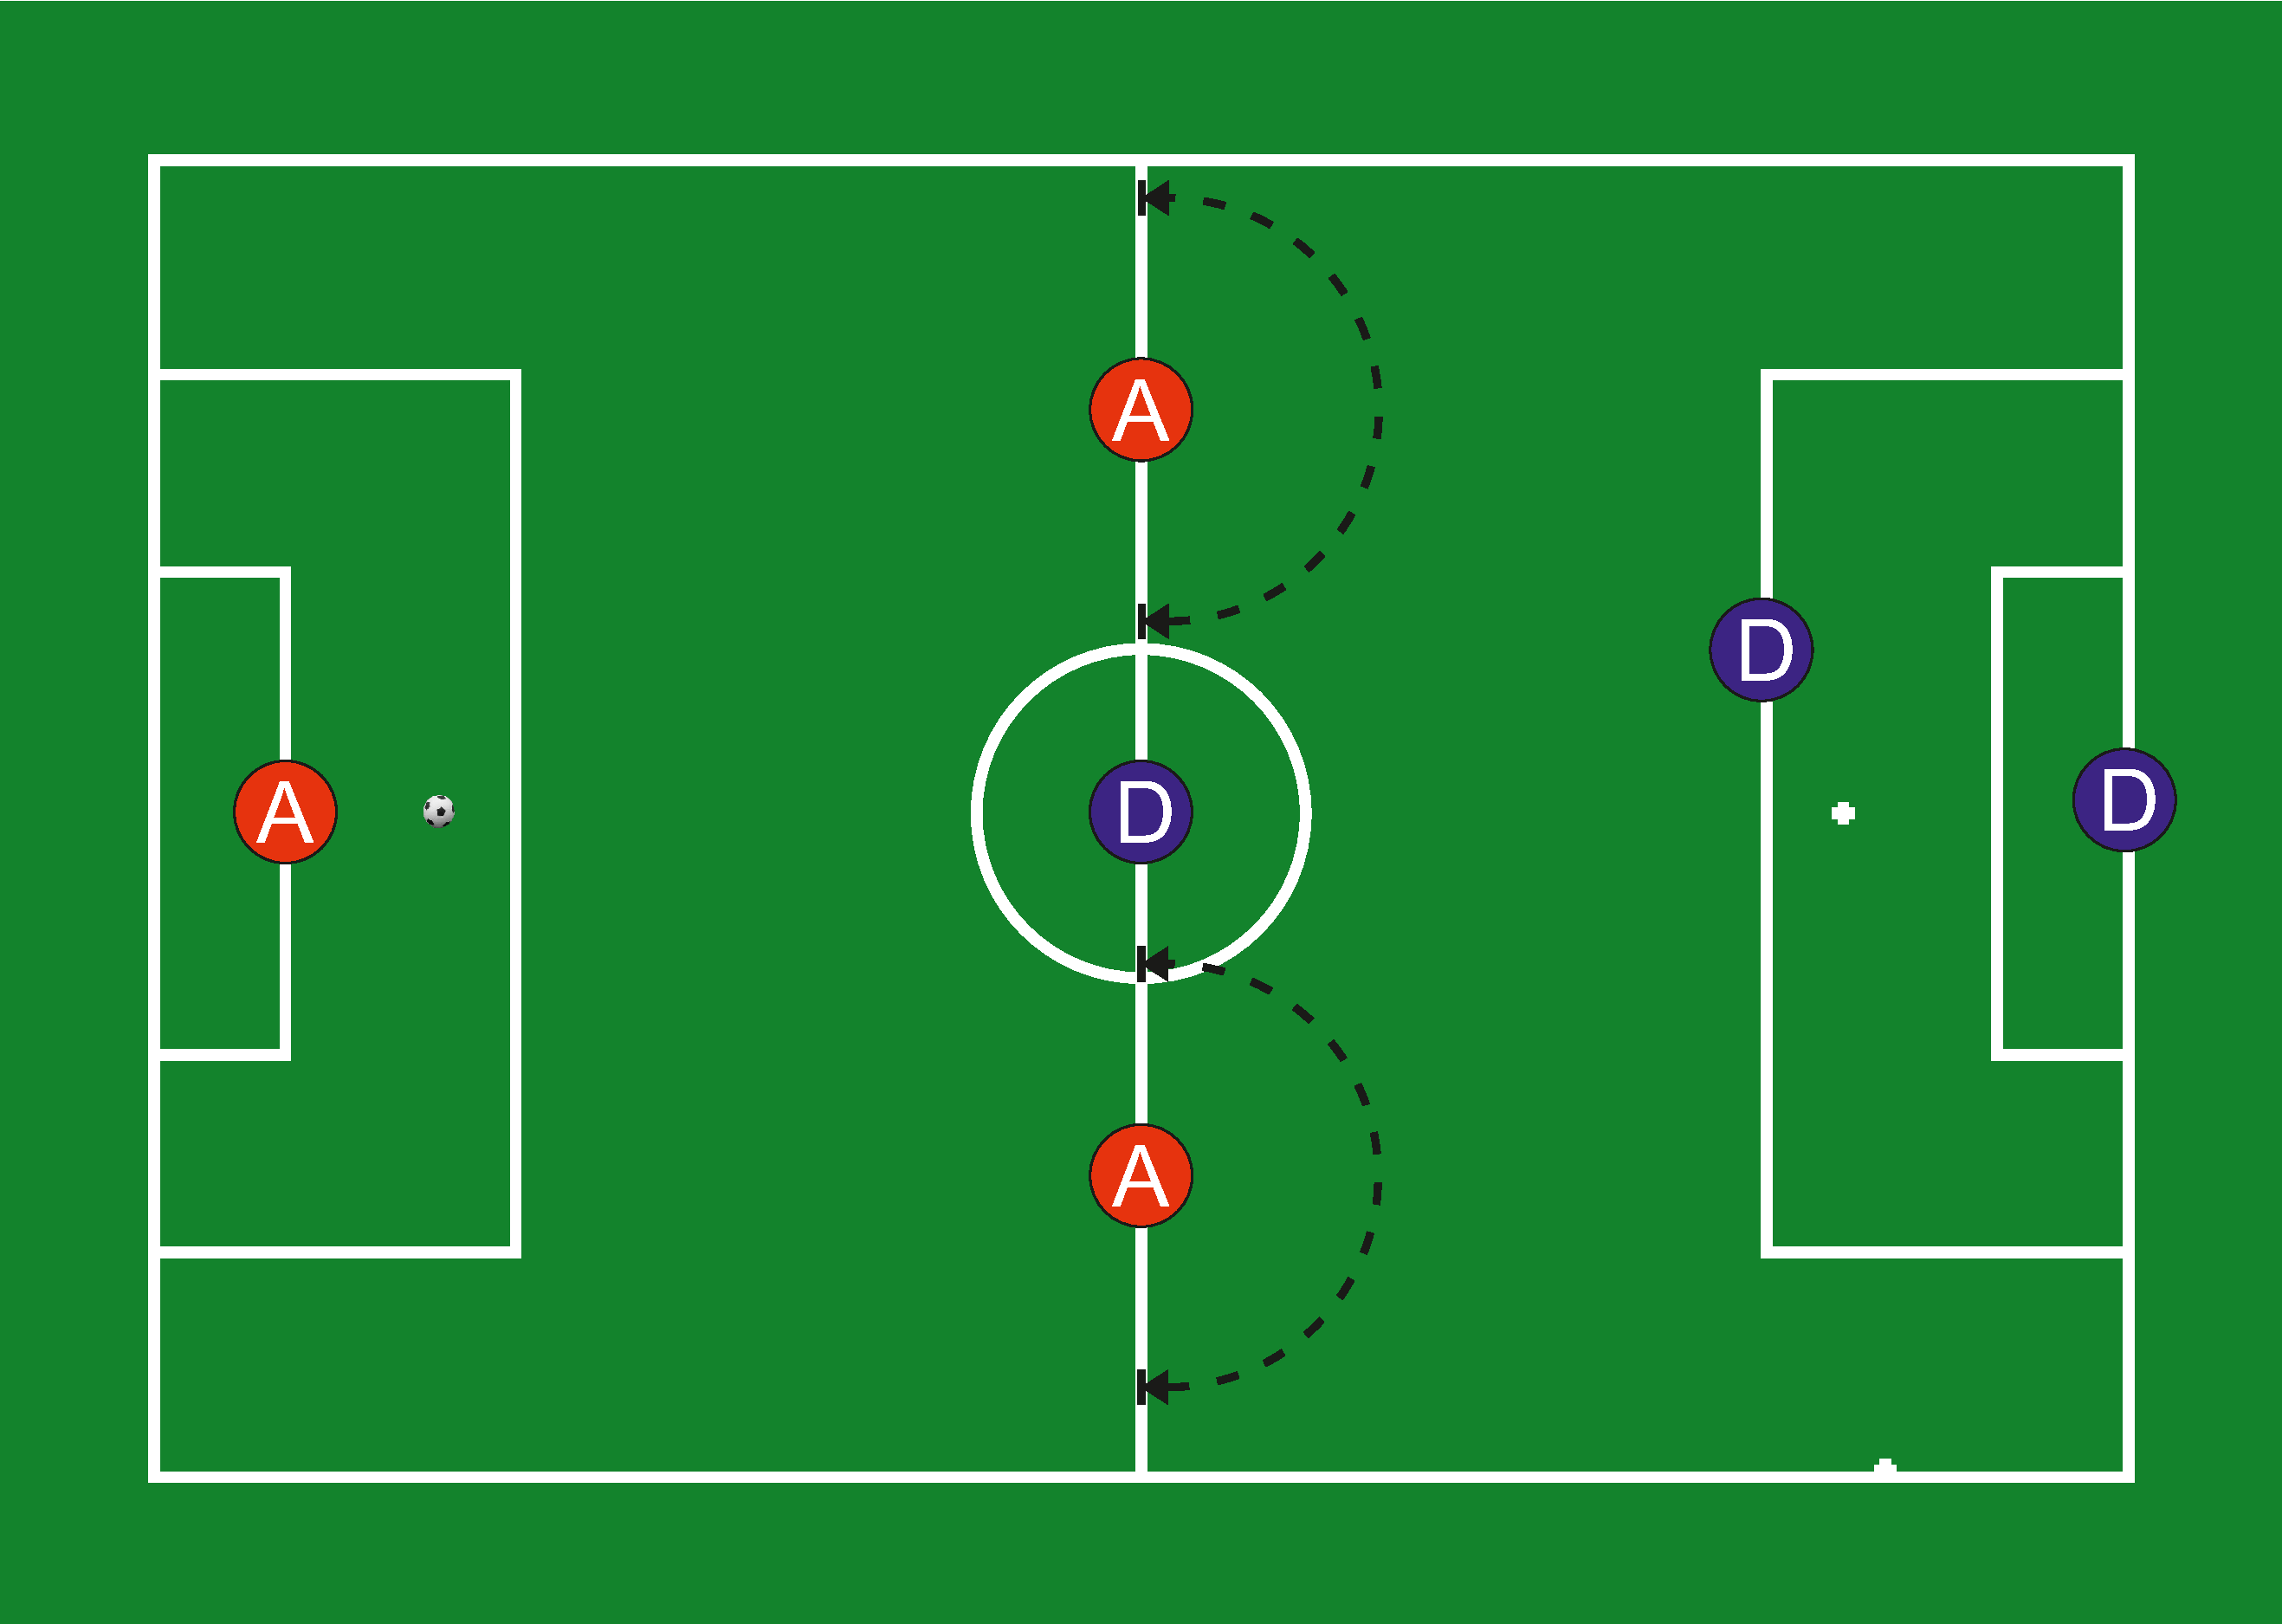
\includegraphics[width=1\columnwidth]{figs/ball_handling_positions.pdf}
                \caption{Possible positions of the attacking (red) and defending (blue) robots at the beginning of the challenge. The black semicircle indicates the area in which a pass is valid.}
                \label{fig:ball_handling_positions}
            \end{center}
        \end{figure}

    Each team has three attempts to run this challenge.

    \subsubsection{Challenge Execution}

        All six robots have to be in the Wi-Fi. In \texttt{initial} the robots get placed at their randomized starting positions. GC goes from \texttt{ready} directly into \texttt{set}. The ball gets placed, and the head referee starts the challenge execution with one whistle, like at kick-off. If a robot does not listen to the whistle, it will get the delayed \texttt{playing} signal from the GC.

        In \texttt{playing} the following happens: The 1st attacker plays the ball towards the 2nd or 3rd attacker while he is under attack by the 1st defender.
        A pass counts as a valid pass if the ball stops in front of the receiving robot towards the opponent's goal. The ball has to stop in the vicinity of the receiving robot (at max \qty{1}{\metre} distance between receiver and ball, see~\cref{fig:ball_handling_positions}).
        The 1st defender does not walk back in its own half and the goalkeeper remains on the goal line and is not allowed to dive. The objective of the defending team is to intercept the passes, see stopping criteria.

        After the 2nd or 3rd attacker received the ball, and the ball is in the defender's half, it gets attacked by the 2nd defender. The task of the 2nd or 3rd attacker is now to pass towards the 3rd or 2nd attacking robot, which than shots onto the goal.

        If a defender pushes an attacking robot, the attacking team gets a time bonus of \qty{15}{\second} and the pushing robot will be removed from this run.

    \subsubsection{Challenge Scoring}

        For each run the referee measures the execution time from initial whistle until the run is stopped by one of the following criteria:

        \begin{itemize}
            \item A defender touches the ball.
            \item Ball leaves the field.
            \item An attacker pushes.
            \item A run exceeds \qty{4}{\minute} execution time.
            \item A goal is scored.
        \end{itemize}

        A score for the run will be calculated based on the following rules:

        \begin{enumerate}
            \item The time measured counts.
            \item If an attacking robot has been pushed by a defender, subtract \qty{15}{\second}.
            \item If a goal has been scored after two passes, subtract \qty{30}{\second}.
            \item If a ball has been passed wrongly, add \qty{10}{\second} for each incorrect pass.
            \item If the ball got touched by the 1st or 2nd defender, execution time will be \qty{240}{\second}.
            \item If the ball leaves the field not from inside the defending goal area, execution time will be \qty{240}{\second}.
            \item If an attacking robot has pushed, execution time will be \qty{240}{\second}.
        \end{enumerate}

        The final result is the mean time out of three runs.

    \subsubsection{Challenge image}
        \label{sec:Challenge_image}
        \todo{Deadline for submission}
        A common image will be provided by the community with the standardized setup procedure and with automatic calibration. Every team can propose such an image \todo{deadline}. The image will be tested if they match the requirements.
        \todo{Criterias for images, how to setup}

\subsection{Open Research Challenge — Video analysis / statistics}
In order to evaluate the progress of the league, regardless of the annual rule changes, we need statistics similar to human soccer. Therefore, only GameController/TeamCom statistics are not sufficient for this. That's why there is an Open Research Challenge, as already known from the year 2019 (and previously until RoboCup 2014), which will focus on the generation of statistics from external video data from a go-pro type camera viewpoint.

    \subsubsection{Challenge Goal}
    For this Open Research Challenge two major goals exist. The more short-term goal is to calculate extrinsic camera parameters (camera matrix) from the camera feed and to locate/track all moving objects (ball, robots) on the field. In addition to this, the more long-term goal involves the creation of game statistics based on the located objects and positions from the short-term goal. Here, the following statistics, among others, might be of interest, such as time under control, shots on goal (successful/unsuccessful), passes and so on. Since this is an open challenge, the decision of what to show (short-term, long-term, parts of it) is, within the scope of the goals aforementioned here, entirely up to the teams. In addition, the execution time for this challenge is also not relevant for the time being whether you process it online or offline to the video stream.

    \subsubsection{Condition for participation}
    \begin{itemize}
    \item In order to compete in this Challenge, teams must notify the TC (\url{rc-spl-tc@lists.robocup.org}) of their interest in participating by 2021-12-31, at the latest.
    \item Subsequently, all participating teams will receive a pre-processed video from the RoboCup2019 (i.e. a sequence of images) and have to label it according to the enclosed instructions. Annotating must be completed by 2022-02-01 to in order to form a shared ground truth data set. However, the final format in which the teams have to submit their annotations has not yet been determined, but the TC is happy to accept suggestions. Also the exact details are given to the teams together with the to be labelled data set.
    \item With this shared ground truth data set, teams can then implement their own approach/ideas. Also any failures in the annotations can be corrected by the community/teams since the data will be shared on the SPL Github\footnote{https://github.com/RoboCup-SPL}.
    \item The teams have to create a poster (A3/A2/A1 size\todo{decide the size}) for the RoboCup 2022 showing their results and prepare a short 3 minutes oral presentation which additionally explains and shows the idea and results of this approach.
    \item All teams are requested to publish the code for their approach to enable a fast progress of the league in this area. However, only the top 3\todo{decide the number} ranked teams are required to publish their code within one month after the RoboCup 2022.
    \end{itemize}

    \subsubsection{Scoring}
    The winner will be decided by a vote among the SPL teams using the Borda count mechanism (\url{http://en.wikipedia.org/wiki/Borda_count}). Each participating SPL team will vote for their top 5/10\todo{decide the number} teams in order (excluding themselves). Teams are encouraged to evaluate the performance based on the following criteria: achievement of the long/short-term goal, execution time, accuracy/precision/recall, technical strength, novelty. At a time decided by the designated referee, within one hour of the last demonstration if not otherwise specified, the captain of each team will submit the team's rankings by filling out an online form. Any points awarded by a team to itself will be disregarded. The points awarded by the teams will be summed and thus form the score of this challenge which is then converted according to the formula described in the beginning of this section.

    \subsubsection{Labelling}
    This section gives a brief overview of the labelling task.\\

    Input data (given):
    \begin{itemize}
        \item The assigned, pre-processed, go-pro videos/sequences from a game of the RC2019.
        \item Additionally the GC data, TeamCom logs and the intrinsic calibration of the go-pro.
    \end{itemize}

    Output data (to be annotated):
    \begin{itemize}
        \item Calculation of the extrinsic camera parameters (camera matrix). Preferably for each frame, although this is mainly necessary when the camera was moved/wobbled. However, it should be checked at least once for each minute whether the camera matrix is still appropriate.
        \item Labelling of all robots and the (main) ball: These objects should be labeled using bounding boxes. Special attention should be paid to the bottom edge as this will be used to determine the position of the object.
        \item In addition, the robots must be labelled with their jersey colour and number.
    \end{itemize}
    Also not everything is fixed yet so that the TC is happy to accept suggestions at \url{rc-spl-tc@lists.robocup.org}.
